\section{样本空间与概率}

\subsection{概率模型}

\begin{definition}[概率模型的基本构成]
概率模型由样本空间和概率律构成:
\begin{itemize}
    \item 样本空间 $\Omega$:一个试验的所有可能结果的集合。
    \item 概率律:为试验结果的集合 $A$(称为事件)确定一个非负数 $\Pb(A)$,称为事件 $A$ 的概率。概率律需要满足概率公理。
\end{itemize}
\begin{figure}[H]
    \centering
    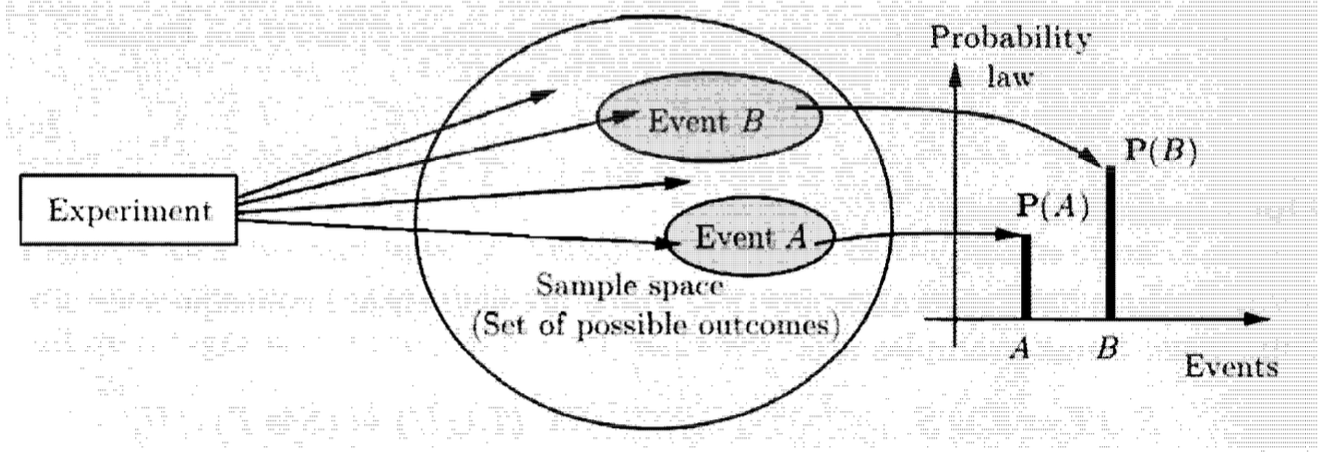
\includegraphics[width=0.8\linewidth]{figs/概率模型的基本构成.png}
    \caption{概率模型的基本构成}
    \label{fig:prob-model-components}
\end{figure}
\end{definition}

\begin{definition}[概率公理]
概率满足以下几条公理:
\begin{enumerate}
    \item 非负性:对一切事件 $A$,满足 $\Pb(A)\geq 0$.
    \item 归一化:整个样本空间为必然事件,即 $\Pb(\Omega)=1$.
    \item 可数可加性:设 $A_1,A_2,\ldots$ 是一列互不相容事件,则 $\Pb(A_1\cup A_2\cup\cdots)=\Pb(A_1)+\Pb(A_2)+\cdots$.
\end{enumerate}
\end{definition}

\begin{property}
设 $A,B,C$ 为事件,则由概率公理可以推导出如下性质:
\begin{itemize}
    \item 空事件概率为 0,即 $\Pb(\varnothing)=0$
    \item $A\subset B\implies \Pb(A)\leq \Pb(B)$
    \item $\Pb(A\cup B)=\Pb(A)+\Pb(B)-\Pb(A\cap B)$
    \item $\Pb(A\cup B)\leq \Pb(A)+\Pb(B)$
    \item $\Pb(A\cup B\cup C)=\Pb(A)+\Pb(A^c\cap B)+\Pb(A^c\cap B^c\cap C)$
\end{itemize}
\end{property}


\subsection{条件概率}

\begin{definition}[条件概率]
设 $A,B$ 为两个事件且 $\Pb(B)>0$,定义 $B$ 发生的条件下 $A$ 发生的概率为:\[\Pb (A\vert B)=\frac{\Pb(A\cap B)}{\Pb(B)},\quad \Pb(B)>0\]
\end{definition}

\begin{theorem}
条件概率是一个公理化定义下的概率,从而概率的所有性质都适用于条件概率。
\end{theorem}
\begin{proof}
只需验证条件概率是否满足非负性、归一化和可数可加性即可。
\begin{enumerate}
    \item 非负性:显然;
    \item 归一化:\[\Pb(\Omega\vert B)=\frac{\Pb(\Omega\cap B)}{\Pb(B)}=\frac{\Pb(B)}{\Pb(B)}=1\]
    \item 可数可加性:
    \begin{align*}
    \Pb\left(\left.\bigcup_{i=1}^nA_i\right\vert B\right)&=\frac{\Pb\left(\left(\bigcup_{i=1}^nA_i\right)\cap B\right)}{\Pb(B)}=\frac{\Pb\left(\bigcup_{i=1}^n(A_i\cap B)\right)}{\Pb(B)}\\
    &=\frac{\sum_{i=1}^n\Pb(A_i\cap B)}{\Pb(B)}=\sum_{i=1}^n\Pb(A_i\vert B)
    \end{align*}
\end{enumerate}
\end{proof}

\begin{theorem}[乘法公式]
设 $A,B$ 为两个事件,则由定义易知:\[\Pb (A\cap B)=\Pb(B)\Pb(A\vert B)\]
\end{theorem}

\begin{corollary}
设 $A_1,A_2,\ldots,A_n$ 为 $n$ 个事件,则:\[\Pb(A_1A_2\cdots A_n)=\Pb(A_1)\Pb(A_2\vert A_1)\Pb(A_3\vert A_1A_2)\cdots\Pb(A_n\vert A_1A_2\cdots A_{n-1})\]
\end{corollary}


\subsection{全概率公式和贝叶斯公式}

\begin{theorem}[全概率公式]
设 $A_1,A_2,\cdots,A_n$ 互不相容,$B\subset A_1\cup A_2\cup\cdots\cup A_n$,则:\[\Pb(B)=\sum_{i=1}^n\Pb(A_i)\Pb(B\vert A_i)\]
\end{theorem}
\begin{proof}
\[\Pb(B)=\Pb\left(B\cap \left(\bigcup_{i=1}^nA_i\right)\right)=\Pb\left(\bigcup_{i=1}^n(A_i\cap B)\right)=\sum_{i=1}^n\Pb(A_i\cap B)=\sum_{i=1}^n\Pb(A_i)\Pb(B\vert A_i)\]
\end{proof}

\begin{theorem}[贝叶斯公式]
设 $A_1,A_2,\cdots,A_n$ 互不相容且 $\Pb(A_i)>0$,$B\subset A_1\cup A_2\cup\cdots\cup A_n$,则:
\[\Pb(A_i\vert B)=\frac{\Pb(A_i\cap B)}{\Pb(B)}=\frac{\Pb(A_i)\Pb(B\vert A_i)}{\sum\limits_{j=1}^n\Pb(A_j)\Pb(B\vert A_j)}\]
其中 $\Pb(A_i)$ 称作先验概率,$\Pb(A_i\vert B)$ 称作后验概率。
\end{theorem}

\begin{remark}[关于贝叶斯公式的理解]
视事件 $A_i$ 是导致事件 $B$ 发生的原因,我们对于事件 $A_i$ 已有一个先验概率 $\Pb(A_i)$,现在事件 $B$ 发生了,这必然给我们带了一定的信息,于是我们可以由此修正 $A_i$ 发生的概率,得到 $\Pb(A_i\vert B)$,即后验概率。
\end{remark}


\subsection{独立性}

\begin{definition}[独立]
设 $A,B$ 是两个事件,称 $A$ 与 $B$ 独立,若:\[\Pb(A\cap B)=\Pb(A)\Pb(B)\]
\end{definition}
\begin{com}
若 $\Pb(B)\neq 0$,则 $A$ 与 $B$ 独立等价于:
\[\Pb(A\vert B)=\Pb(A)\]
直观上,这说明事件 $B$ 的发生与否并不给 $A$ 带来信息,不改变 $A$ 发生的概率。
\end{com}
\begin{note}
事件的独立性常常不能直观地看出来。例如,若事件 $A$ 与事件 $B$ 互不相容,并且 $\Pb(A)>0,\,\Pb(B)>0$,则它们一定不独立,因为 $\Pb(A\cap B)=0\neq\Pb(A)\Pb(B)$. 直观上,事件 $B$ 发生意味着 $A$ 一定没有发生,因此 $B$ 的发生与否会给 $A$ 带来信息。
\end{note}

\begin{theorem}
设事件 $A$ 与事件 $B$ 独立,则 $A$ 与 $B^c$ 也独立。
\end{theorem}
\begin{proof}
由于 $A$ 可写作两个不相容事件之并 $A=(A\cap B)\cup (A\cap B^c)$,故:
\[
\Pb(A)=\Pb(A\cap B)+\Pb(A\cap B^c)
\]
于是:
\[
\Pb(A\cap B^c)=\Pb(A)-\Pb(A\cap B)=\Pb(A)-\Pb(A)\Pb(B)=\Pb(A)(1-\Pb(B))=\Pb(A)\Pb(B^c)
\]
\end{proof}

\begin{definition}[条件独立]
给定事件 $C$,称事件 $A,B$ 在给定 $C$ 下条件独立,若:
\[\Pb(A\cap B\vert C)=\Pb(A\vert C)\Pb(B\vert C)\]
\end{definition}
\begin{com}
$A,B$ 条件独立并不能推出 $A,B$ 独立,反之亦不成立。
\end{com}

\begin{definition}[一组事件的相互独立性]
设 $A_1,A_2,\ldots,A_n$ 是一组事件,称它们相互独立,若:
\[
\Pb\left(\bigcap_{i\in S}A_i\right)=\prod_{i\in S}\Pb(A_i),\quad\forall S\subset\{1,2,\ldots,n\}
\]
\end{definition}
\begin{note}[两两独立与相互独立]
设 $A_1,A_2,A_3$ 相互独立,则有:
\begin{gather*}
\Pb(A_1\cap A_2)=\Pb(A_1)\Pb(A_2)\\
\Pb(A_2\cap A_3)=\Pb(A_1)\Pb(A_3)\\
\Pb(A_1\cap A_3)=\Pb(A_1)\Pb(A_3)\\
\Pb(A_1\cap A_2\cap A_3)=\Pb(A_1)\Pb(A_2)\Pb(A_3)
\end{gather*}
前三个式子称作两两独立。但是第四个式子也非常重要,它并不是前三个式子的推论;反之,第四个式子也不能推出前三个式子。
\end{note}
\begin{example}[两两独立不能推出独立]
设试验是抛掷两枚均匀的硬币,考虑事件:
\[H_1=\{\text{第一次正面}\},\quad H_2=\{\text{第二次正面}\},\quad D=\{\text{两次结果不同}\}\]
则易知 $H_1$ 与 $H_2$ 独立。另外,
\[
\Pb(D\vert H_1)=\frac{\Pb(D\cap H_1)}{\Pb(H_1)}=\frac{1/4}{1/2}=\frac{1}{2}=\Pb(D)
\]
故 $D$ 与 $H_1$ 独立。同理可知 $D$ 与 $H_2$ 独立,故 $H_1,H_2,D$ 两两独立。但是:
\[
\Pb(H_1\cap H_2\cap D)=0\neq \Pb(H_1)\Pb(H_2)\Pb(D)=\frac{1}{2}\cdot\frac{1}{2}\cdot\frac{1}{2}
\]
故 $H_1,H_2,D$ 不是独立的。
\end{example}
